\documentclass[UTF8,aspectratio=169,11pt,fontset=fandol]{ctexbeamer}
\usepackage{booktabs,amsmath,graphicx,tikz}
\definecolor{deep}{HTML}{111D22}\definecolor{green}{HTML}{216B62}\definecolor{paper}{HTML}{F5F4EE}\definecolor{mint}{HTML}{A6D9BC}\definecolor{ochre}{HTML}{B56D47}
\setbeamercolor{background canvas}{bg=paper}\setbeamercolor{normal text}{fg=deep}\setbeamercolor{frametitle}{fg=green}\setbeamercolor{structure}{fg=green}
\setbeamertemplate{navigation symbols}{}\setbeamertemplate{footline}{\hspace{6mm}\tiny 梁鉴 / AI+力学开放式赛题\hfill 仿真研究原型\hspace{6mm}\insertframenumber\hspace{6mm}\vspace{4mm}}
\setbeamertemplate{frametitle}{\vspace{5mm}\insertframetitle\par\vspace{2mm}{\color{green}\hrule}}
\setbeamersize{text margin left=9mm,text margin right=9mm}
\newcommand{\HybridMAE}{0.135}
\newcommand{\PhysicsMAE}{0.150}
\newcommand{\AIMAE}{0.757}
\newcommand{\HybridTime}{21.6}
\newcommand{\PhysicsTime}{81.7}
\newcommand{\AITime}{3.9}
\newcommand{\Speedup}{3.78}
\newcommand{\CallSaving}{80.2}
\newcommand{\Coverage}{87.5}
\newcommand{\Width}{2.08}
\newcommand{\Accept}{97.5}
\newcommand{\HealthyFalseAblation}{44.2}
\newcommand{\MeshMAE}{0.128}
\newcommand{\TripleMAE}{4.77}
\newcommand{\MassMAE}{5.51}
\newcommand{\NoiseMAE}{0.801}
\newcommand{\FullSeconds}{128.8}
\newcommand{\HybridDamagedMAE}{0.517}

\title{梁鉴：环境扰动下的损伤识别}\author{}\date{2026年10月13日}
\begin{document}
{\setbeamercolor{background canvas}{bg=deep}\setbeamercolor{normal text}{fg=paper}\usebeamercolor[fg]{normal text}
\begin{frame}[plain]
\vspace{7mm}{\color{mint}\small AI + MECHANICS\quad /\quad AIC 2026}\par\vspace{10mm}
{\fontsize{34}{42}\selectfont 梁鉴}\par\vspace{5mm}
{\fontsize{23}{30}\selectfont 环境扰动下的损伤识别}\par\vspace{9mm}
{\color{mint}AI筛选候选位置\quad /\quad 物理反演与独立模态校核}\par\vfill
{\small 六分区悬臂梁 · 720个独立仿真测试工况\hfill 团队编号待补}\vspace{6mm}
\end{frame}}
\begin{frame}{01\quad 同样是频率下降，原因可能不同}
\begin{columns}[T]\column{.46\textwidth}
\vspace{5mm}{\Large 环境变化}\par\vspace{4mm}$K=\alpha K_0$\par\vspace{4mm}
频率统一乘以$\sqrt\alpha$，\par 归一化振型不变。
\column{.46\textwidth}\vspace{5mm}{\Large 局部损伤}\par\vspace{4mm}$K=\alpha\sum_j(1-d_j)K_j^0$\par\vspace{4mm}
不同分区改变不同模态，\par 但变化可能很小。
\end{columns}\vspace{12mm}
{\color{ochre}必须承认：均匀损伤与整体模量变化，仅凭模态不可辨识。}\par\vspace{3mm}\small 研究范围限定为已知健康参考、少数局部损伤的教学与试验梁。
\end{frame}
\begin{frame}{02\quad AI负责缩小搜索，力学负责估计参数}
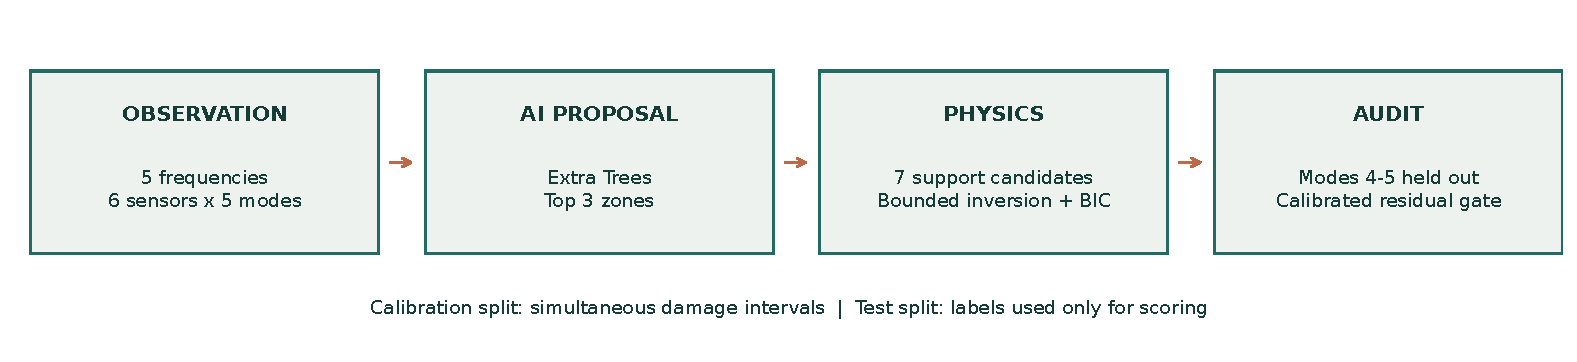
\includegraphics[width=\linewidth]{generated/workflow.pdf}\vspace{5mm}
\begin{columns}[T]\column{.32\textwidth}\textbf{AI提议}\par\small 160棵极端随机树\par 取三个候选分区
\column{.32\textwidth}\textbf{物理反演}\par\small 22个支持集缩减为7个\par 有界求解与BIC型选择
\column{.32\textwidth}\textbf{独立检查}\par\small 第4、5阶不参与拟合\par 只校核，不回流调参
\end{columns}\vspace{5mm}\small 贡献为问题建模、融合与校核流程；基础算法来自已有方法。
\end{frame}
\begin{frame}{03\quad 模型和每一个量都能校核}
\begin{columns}[T]\column{.52\textwidth}\vspace{3mm}
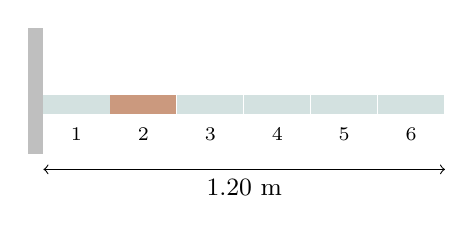
\begin{tikzpicture}[x=1cm,y=1cm]
\fill[gray!50](-.2,-.5)rectangle(0,1.1);
\foreach \zone in {0,...,5}{\pgfmathtruncatemacro{\labelnum}{\zone+1}\fill[green!20](\zone*.85,0)rectangle(\zone*.85+.84,.25);\node at(\zone*.85+.42,-.25){\scriptsize\labelnum};}
\fill[ochre!70](.85,0)rectangle(1.69,.25);\draw[<->](0,-.7)--node[below]{\small1.20 m}(5.1,-.7);
\end{tikzpicture}\par\small 六分区，12个梁单元；左端固支\par 截面30 mm$\times$6 mm，$E=70$ GPa
\column{.44\textwidth}\vspace{3mm}
$K\phi=\omega^2M\phi$\par\vspace{4mm}\small
解析频率\quad 端部静挠度\par\vspace{2mm}
质量正交\quad 特征方程残差\par\vspace{2mm}
环境缩放\quad 网格收敛\par\vspace{5mm}
\textbf{10项测试全部通过。}
\end{columns}\vspace{9mm}\small 梁假设：线弹性、小变形、已知质量和理想夹持。损伤指刚度折减，非裂纹深度。
\end{frame}
\begin{frame}{04\quad 同输入、强基线、独立数据}
\vspace{4mm}\begin{columns}[T]
\column{.29\textwidth}{\fontsize{30}{36}\selectfont 3}\par\vspace{2mm}\small 独立模型种子
\column{.29\textwidth}{\fontsize{30}{36}\selectfont 720}\par\vspace{2mm}\small 独立测试工况
\column{.36\textwidth}{\fontsize{30}{36}\selectfont 2880}\par\vspace{2mm}\small 逐方法预测记录
\end{columns}\par\vspace{5mm}
\begin{tabular}{p{36mm}p{90mm}}\toprule
训练与校准 & 每种子2400训练、120校准；不同随机流\\[2mm]
测试 & 6域各40例/种子；常规、健康、噪声、网格、三损伤、附加质量\\[2mm]
比较对象 & 纯AI；22候选穷举反演；忽略环境消融\\[2mm]
复现 & 第二遍从数据生成开始重训，非计时结果全部一致\\\bottomrule
\end{tabular}\par\vspace{3mm}\small 全部为合成模态特征，尚未经过原始传感器波形或实物验证。
\end{frame}
\begin{frame}{05\quad 相近误差，减少在线搜索开销}
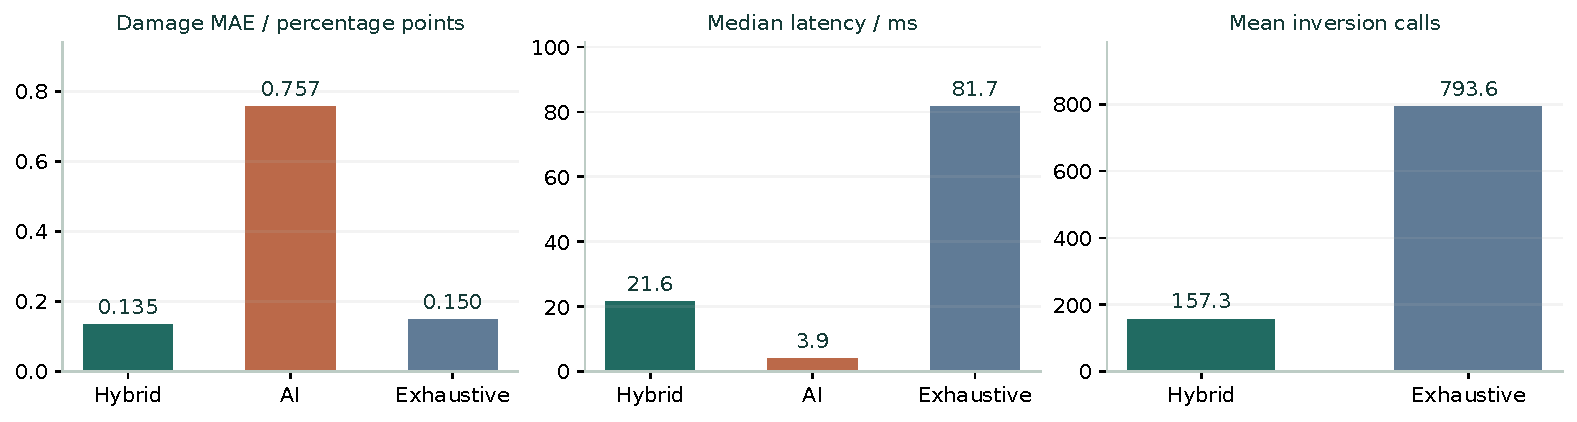
\includegraphics[width=\linewidth]{generated/headline.pdf}\vspace{3mm}
\begin{columns}\column{.48\textwidth}{\Large\color{green}\Speedup 倍}\par\small 穷举/融合在线中位耗时之比
\column{.48\textwidth}{\Large\color{green}\CallSaving\%}\par\small 前向调用减少比例
\end{columns}\vspace{3mm}\small 常规域120例；融合MAE \HybridMAE、穷举\PhysicsMAE 个百分点。计时含在线AI推理，不含离线训练；未声称精度显著优于穷举。
\end{frame}
\begin{frame}{06\quad 误差区间与失配，都需要展示}
\centerline{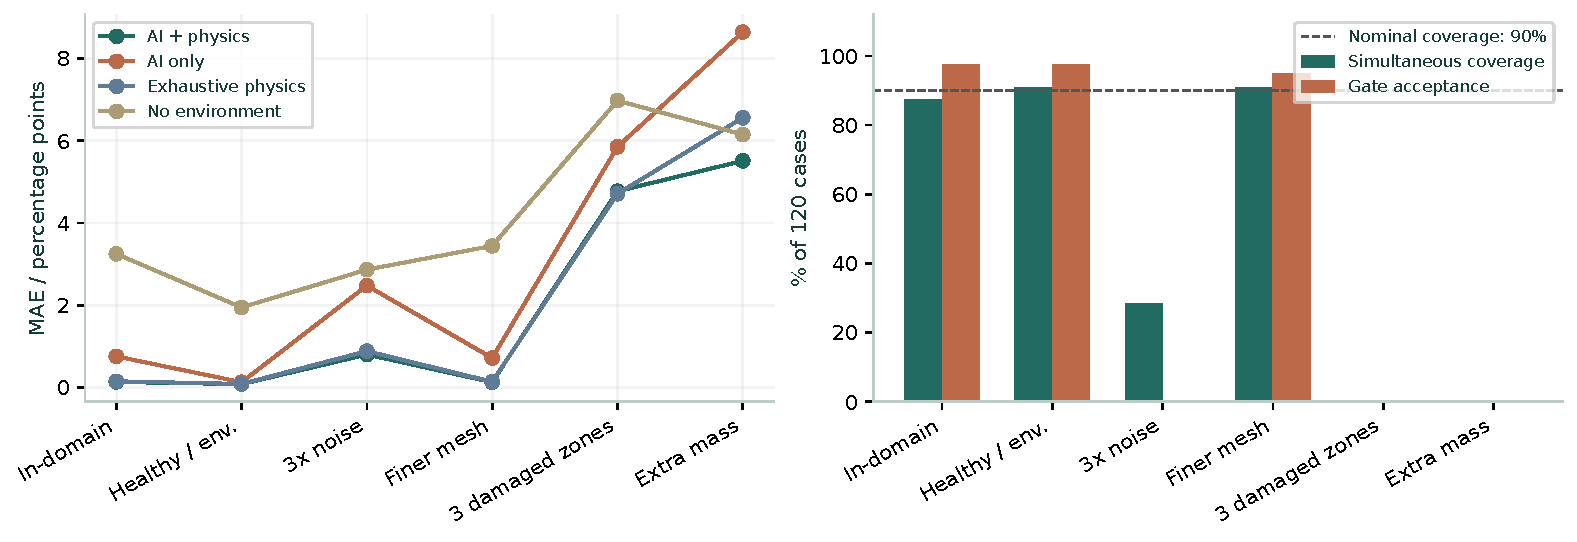
\includegraphics[width=.93\linewidth]{generated/robustness.pdf}}\vspace{2mm}
\small 常规域标称90\%的同时区间，实测覆盖\Coverage\%。\par
\vspace{2mm}\color{ochre}高噪声、三处损伤和附加质量各120例均触发复核；\par 这不能推出对任意未知异常均可检测。
\end{frame}
\begin{frame}{07\quad 可视化对应同一组计算结果}
\begin{columns}[T]\column{.62\textwidth}\vspace{3mm}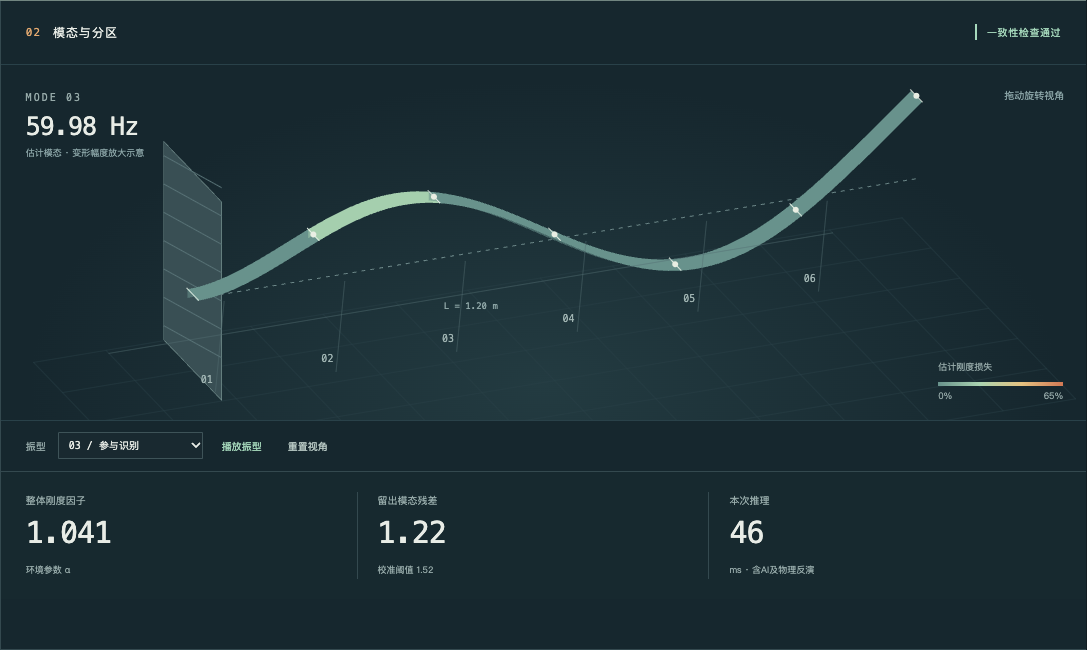
\includegraphics[width=\linewidth,height=43mm,keepaspectratio]{generated/demo_stage.png}\par\vspace{2mm}\tiny 有限元Hermite插值；动画放大振幅、放慢时间，仅用于形态解释。
\column{.34\textwidth}\vspace{3mm}\textbf{现场演示顺序}\par\vspace{4mm}\small
1. 常规域：检查损伤与真值\par\vspace{3mm}
2. 健康梁：分离环境因子\par\vspace{3mm}
3. 附加质量：显示复核提示\par\vspace{3mm}
4. 查看逐分区区间和原始记录
\end{columns}
\end{frame}
\begin{frame}{08\quad 应用价值与下一步验证}
\begin{columns}[T]\column{.45\textwidth}\vspace{4mm}\textbf{当前可用}\par\vspace{5mm}\small
教学演示：模态、损伤和环境混淆\par\vspace{3mm}
算法研究：强基线与失配测试\par\vspace{3mm}
本地复算：模型、数据、原始记录
\column{.5\textwidth}\vspace{4mm}\textbf{下一步实物试验}\par\vspace{5mm}\small
核验健康梁参数、夹持与模态\par\vspace{3mm}
记录温度、质量及重复测量\par\vspace{3mm}
冻结校准，预留独立损伤工况
\end{columns}\vspace{9mm}\color{ochre}当前不提供结构安全鉴定，也不虚构经济收益、专利或合作证明。
\end{frame}
{\setbeamercolor{background canvas}{bg=deep}\setbeamercolor{normal text}{fg=paper}\usebeamercolor[fg]{normal text}
\begin{frame}[plain]\vspace{8mm}{\color{mint}\small 梁鉴 / BEAM INSIGHT}\par\vspace{10mm}
{\fontsize{29}{38}\selectfont 从一个预测，\par 到一条可复核的证据链。}\par\vspace{9mm}
\small 稀疏损伤假设\quad →\quad AI候选\quad →\quad 力学反演\quad →\quad 独立校核\par\vspace{10mm}
{\color{mint}源码、模型、逐例记录、反例与复现命令完整保留。}\par\vfill
\small 参考：Peeters et al. (2001)；Angelopoulos \& Bates (2021)。\par 团队编号与人工审核待补。AI辅助范围见\texttt{docs/AI\_USE.md}。\vspace{5mm}
\end{frame}}
\end{document}
